% !TEX root = main.tex

\section{はじめに}

\section{関連研究}
\label{sec:relatedwork}
関連の深い索引構造として,同時実行制御においてロックを取得しない\Bctree{},および\Bptree{}にトライ木の構造を組み合わせたMass木について紹介する.

\subsection{\Bctree{}}
\Bctree{}はマッピングテーブル,ノード内バッファという構造上の特徴とCAS命令を用いたロックフリー索引である.
\Bctree{}の概形を\Fig{\ref{fig:bc_tree-structure}}に示す.

\begin{figure*}[t]
    \centering
    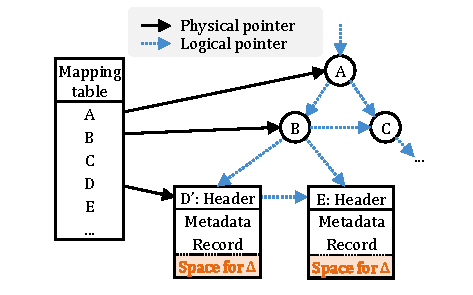
\includegraphics{./figures/Bc-structure.pdf}
    \caption{\Bctree{}の概形}
    \label{fig:bc_tree-structure}
\end{figure*}

\subsubsection{木構造}
マッピングテーブルはノード間のリンクを仮想化し,メインメモリ上の差分更新を可能とする.
各ノードは自身の子ノードや兄弟ノードへのポインタを直接持つ代わりにマッピングテーブル上のID(logical page ID, LPID)を持つ.
各ノードへの参照はマッピングテーブルを用いた間接参照を採用し,マッピングテーブル内の物理ポインタを差し替えることでそのノードへの参照を一括で変更する.

\Bptree{}と同様に,\Bctree{}は索引層およびデータ層によって構成される.
索引層のノード(中間ノード)は分割キーと子ノードへのポインタの組を格納し,木の下方への検索を補助する.
構造は\Blinktree{}に則っており,各ノードが同じ階層の右兄弟への参照リンクを持つ.

\subsubsection{ノード構成}
各ノードの領域はイミュータブル領域とミュータブル領域(ノード内バッファ)に分けられる.

イミュータブル領域はノードヘッダおよびソート済みのレコードを格納する.
ヘッダはイミュータブル領域の情報を管理し,構造変更時のみその値が変更される.

ミュータブル領域はステータスワードの格納と差分レコードを挿入するための書き込みバッファの役割を果たす.
ステータスワードはミュータブル領域の情報を管理し,ノードの現在の状態や残容量などを管理する.
ステータスワードをCAS命令で更新することによって,ロックフリーな書き込みを実現している.
各ノードへ構造変更操作を行う際は,構造変更後のノードから構造変更前のノードへ物理リンクを張り,古いノードへの参照を可能にする.
なお,古いノードは構造変更が済み次第,ガベージコレクションへ追加され,他のスレッドから参照されないことが保証された時点で削除される.

\subsection{Mass木}
Mass木は\Bptree{}を基本単位とした階層構造を作り,キャッシュ効率を改善した索引構造である.
Mass木の概形を\Fig{\ref{fig:masstree}}に示す.

\begin{figure}[t]
    \centering
    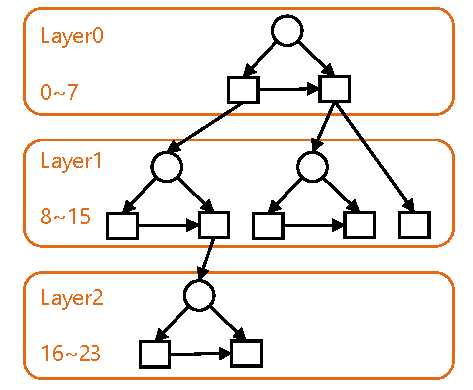
\includegraphics{./figures/masstree.pdf}
    \caption{Mass木の概形}
    \label{fig:masstree}
\end{figure}

Mass木は複数の\Bptree{}とlayer構造から構成される.
Layer0はキーの先頭0~7~byteで構成される\Bptree{}である.
先頭8~byteで一意性が確保できる場合には,Layer0で完結する.
先頭8~byteで一意性が確保出来ない場合,Layer1を作成し,Layer0からLayer1への物理リンクを張る.
Layer1はキーの先頭8~15~byteで構成される\Bptree{}の集合ある.
例えば,Layer0に「aaaaaaaab」をキーとするレコードが格納されており,そこに「aaaaaaaac」をキーとするレコードが書き込まれるとする.
この場合,Layer0には「aaaaaaaa」をキーとし,Layer1へのポインタをペイロードとして持つレコードが格納される.
Layer1には新たに\Bptree{}作成され,「b」をキーとするレコードと「c」をキーとするレコードが格納される.
つまり,同じ接頭辞キー「aaaaaaaa」持つ\Bptree{}が生成される.
同様にして,複数の\Bptree{}やLayerを作成し,トライ木に似た構造を持つのがMass木の特徴である.

Mass木は整数型や文字列型など,分割が可能なキーに限定している.
これにより,上記に示す階層化(共通部分の集約)が可能になり,キャッシュ効率を改善している.

\section{\Bcforest{}の構造}
\label{sec:bc_forest_structure}

\Bcforest{}はBc木をバイナリ比較可能なキーに最適化した索引構造である.
Mass木のように8バイト単位でキーを分割,階層分けし,各階層でのレコード管理にはBc木を利用する.
つまり,各Bc木の中間ノードでは固定長の部分キーおよび子ノードへのポインタのみを管理することとなり,レコードメタデータの除外によるキャッシュ効率の改善が可能となる.
一方で,葉ノードではposting listを用いて共通する部分キーを持つレコードを管理し,少数のレコードのみからなる下層の生成を抑制する.

\subsection{トライ木構造の適応}

Mass木は\Bptree{}にトライ木構造を適応させることで,キャッシュ効率を改善させた.
\Bcforest{}では\Bctree{}に対し,同様の改善を図る.

Mass木の観点では\Bptree{}から\Bctree{}になることにより,ロックフリーによる書き込み性能の改善を図る.
また\Bctree{}の観点では,整数型や文字列型などのバイナリ比較可能なキーに対し,キャッシュ効率の改善を図る.

\subsection{posting listの導入}

\begin{figure*}[t]
    \centering
    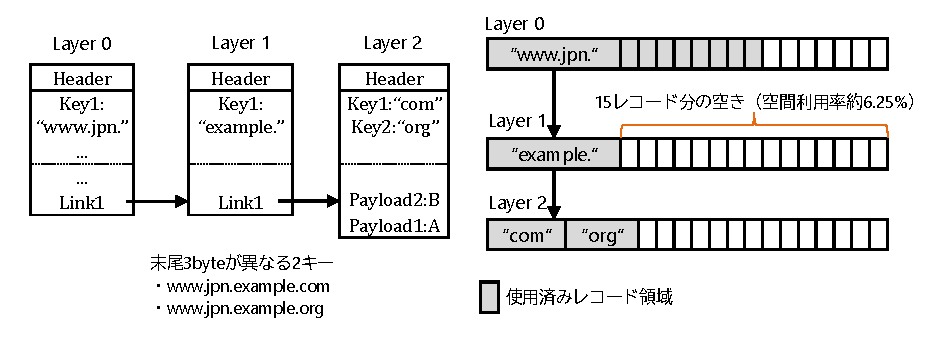
\includegraphics{./figures/memory.pdf}
    \caption{Mass木の空間利用率}
    \label{fig:memory}
\end{figure*}

Mass木においては,空間利用効率が問題となる.
\Fig{\ref{fig:memory}}は末尾3~byteが異なる19~byteの2~キーを格納したMass木の索引構造である.
先頭8~byteが共通するため,layer1を作成する.
同様に8~16~byte目が共通するため,layer2を作成する.
Mass木では本来,1~つのノードに最大16~個のレコードを格納することが出来る.
しかしlayer1では,1~つのレコードしか格納されていない状態でlayer2を作成している.
layer1にのみ注目すると,空間利用率は約6.25~\%しかない.

\begin{figure}[t]
    \centering
    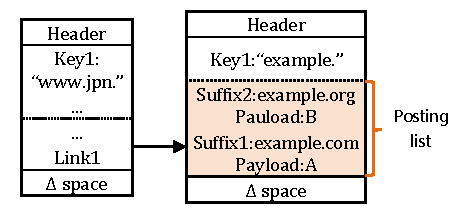
\includegraphics{./figures/posting_list.pdf}
    \caption{posting listの導入}
    \label{fig:posting_list}
\end{figure}

\Bcforest{}では空間利用率の改善として,posting listを導入する.
posting listでは,1~つのキーに対して複数のペイロードを対応付けることが出来る.
\Fig{\ref{fig:posting_list}}はposting listを導入した際の索引構造を示したものである.
layer1においてposting list作成することで,layer2の無駄な階層化と空間利用率の悪化を防ぐ.


\section{\Bcforest{}のノード操作}
\label{sec:node_operation}

\subsection{書き込み}

\subsection{読み取り}

\section{\Bcforest{}の構造変更操作}
\label{sec:smo}

\subsection{統合}
\subsection{分割}
\subsection{新層作成}

\section{おわりに}
\label{sec:conclusion}

